\begin{enumerate}[label=\thesubsection.\arabic*,ref=\thesubsection.\theenumi]

 \hfill\begin{minipage}{\linewidth}
 \item A fair six-faced dice, with the faces labelled ‘1’, ‘2’, ‘3’, ‘4’, ‘5’, and ‘6’, is rolled
    thrice. What is the probability of rolling ‘6’ exactly once?\hfill(GATE AG 2025)
 \begin{enumerate}
    \item[(A)] $\frac{75}{216}$ \vspace{0.1cm}
    \item[(B)] $\frac{1}{6}$\vspace{0.1cm}
    \item[(C)] $\frac{1}{18}$\vspace{0.1cm}
    \item[(D)] $\frac{25}{216}$
\end{enumerate}
\end{minipage}
\bigskip\\Solution:\\
     The sample space is S $\in \{1,2,3,4,5,6\}$ \\
     Let us define a variable $Y_1$ as follows: 
     \begin{align}
         Y_1=
            \begin{cases}
                1&X_1=6\\
                0&X_1\neq6
            \end{cases}
     \end{align}
     Now, The PMF is defined as:\\
        \begin{align}
            P_{Y_1}(k)=
                \begin{cases}
                    \frac{1}{6} &  k=1 \\
                    \frac{5}{6} & k=0\\
                \end{cases}\\\\
            \text{Let p,q be $\frac{1}{6}$ and $\frac{5}{6}$ respectively.}
        \end{align}\\
        
    %\noindent Step 2: Applying Z-Transform to find the required PMF for Y \\\\
    Let us define $Y_2$ and $X_3$ as the random variables for the 2\textsuperscript{nd} and 3\textsuperscript{rd} dice roll, respectively. Let $Y$ denote the random variable for the combined triple dice roll.\medskip\\
    Now, we can write $Y=Y_1+Y_2+Y_3$.\medskip\\
    Writing the Z-Transform (Refer to \eqref{eq:ztransform}) for $Y$\\
        \begin{align}
                 M_{Y_1}(Z)&=\brak{P_{Y_1}(1)Z^{-1} +P_{Y_1}(0)Z^{-0}}\\
                           &=pZ^{-1}+q
        \end{align}
    We know that $Y_1,Y_2,Y_3$ are independent events. So,
    \begin{align}
    M_Y\brak{Z}&=M_{Y_1}\brak{Z}\,\, M_{Y_2}\brak{Z}\,\,M_{Y_3}\brak{Z}\tag{Refer \eqref{eq:ztransformindep}}\\
        M_Y\brak{Z}&=\brak{pZ^{-1}+q}^3\tag{From 7}.\\
              &=\sum_{k=0}^3{^3}C_k\,\,q^{3-k}\,\, \brak{pZ^{-1}}^k\\    
              &=\sum P_Y\brak{k}Z^{-k}\tag{From 5}\\
        \text{So, we can say:}\\
            P_Y\brak{k}&=^3C_k\,\,q^{3-k}\,\,p^k
    \end{align}
    The above situation is called as a binomial distribution.\\
    %\noindent Step 3: Using binomial distribution to get required probability
    We need the situation where p appears exactly once. So, we consider only the term where the power of p is 1.\\
    The required term is :  $^3C_1\,\,p\,\,q^2$.\\
    Substituting the values of p and q, we get:\\
    \begin{center}
        $^3C_1\,\frac{1}{6}\,\,\brak{\frac{5}{6}}^2$\medskip\\
        $=\frac{75}{216}$
    \end{center}
    Therefore, the required answer is $\frac{75}{216}$\medskip\\
\large\underline{C Implementation }:
\begin{lstlisting}
codes/Probability.c
\end{lstlisting}



\hfill\begin{minipage}{\linewidth}
	\item If a, b, and c are the roots of $2x^3 - 3x^2 + px - 1=0$ and sum of the two roots is 1, the value of $p$ is:\hfill(GATE AG 2025)
\begin{enumerate}
    \item[(A)] 2
    \item[(B)] 1
    \item[(C)] 3
    \item[(D)] $\frac{1}{3}$
\end{enumerate}
\end{minipage}
    {Solution}\medskip\\
    \begin{enumerate}
  	\item
    Let the roots whose sum is 1 be $a$ and $b$.\\
    Then, by using the properties of coefficients of an equation, we write:\medskip\\
    \begin{align}
        -\brak{\frac{-3}{2}}&=a+b+c\\
                               \frac{3}{2} &=1+c\\
                               c&=\frac{1}{2} 
    \end{align}
    And
    \begin{align}
        abc&=-\brak{\frac{-1}{2}}\\
        ab\,\frac{1}{2}&=\frac{1}{2}\tag{From 3}\\ 
        ab&=1
    \end{align}
    Also,
    \begin{align}
        ab+bc+ac&=\brak{\frac{p}{2}}\\
        1+c(a+b)&=\frac{p}{2}\tag{From 5}\\
        1+\frac{1}{2}(1)&=\frac{p}{2}\tag{From 3}\\
        3=p
    \end{align}
    Therefore, the value of $p$ is 3.
    \bigskip
    \item
    calculating the roots by newton-raphson method:\\
    given cubic equation is :$2x^3-3x^2+3x-1$\\
    Therefore, the update equation is:\\
    $x_{n+1}=x_n+\frac{2x^3-3x^2+3x-1}{6x^2-6x+3}$
    with an initial guess of 4,running this update equation 6 times gives us the real root, which is $\frac{1}{2}$
    \begin{figure}[htbp]
    \centering
    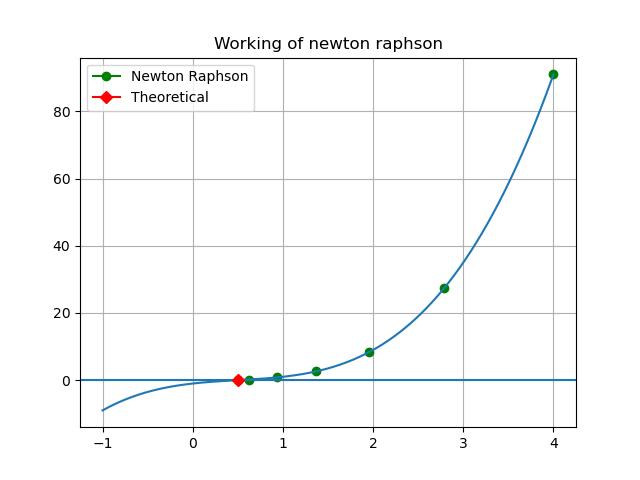
\includegraphics[width=0.7\textwidth]{figs/rson.png}
    \caption{The depiction of newton raphson method guessing the root}
    \label{Plot of the function approaching the limit}
\end{figure} \newpage 

\end{enumerate}
\large\underline{Python Implementation }:
\begin{lstlisting}
\codes\raph.py
\end{lstlisting}


\hfill\begin{minipage}{\linewidth}
\item If the matrix $\myvec{ x & -3 \\ 2 & x-5 }$ is singular, sum of the values of $x$ is:     \hfill(GATE AG 2025)   
    \begin{enumerate}
    \item[(A)] 5
    \item [(B)]6
    \item [(C)] 0
    \item [(D)]$-1$
\end{enumerate}
\end{minipage}
\bigskip\\
Solution\medskip\\
A matrix is said to be singular if its row echelon form has a row full of zeroes.\medskip\\
Finding row echelon form of the given matrix:\medskip\\
\begin{center}
      $\myvec{
        x&-3\\
        2&x-5 
        }$\bigskip\\
        $\myvec{
        x&-3\\
        1&\frac{(x-5)}{2} 
         }$\bigskip\\
        $\myvec{
        x-x\cdot1&\frac{-6-(x-5)}{2}\\
        1&\frac{\brak{x-5}}{2} 
        }$\bigskip\\
        $\myvec{
        0&\frac{\brak{-6-x^2+5x}}{2}\\
        1&\frac{\brak{x-5}}{2} 
        }$\bigskip\\
        $\myvec{
        1&\frac{\brak{x-5}}{2}\\
        0&\frac{\brak{-6-x^2+5x}}{2}
        }$\bigskip\\  
\end{center}
%\noindent Step 2: Making the bottom row to be full of zeroes:\medskip\\
We need to equate $\frac{\brak{-6-x^2+5x}}{2}$ to zero.\\
We get 
\begin{align}
    -6-x^2+5x=0\\
    x^2-5x+6=0
\end{align}
So, the sum of values of $x$ is 5.\medskip\\
The following code converts a numerical matrix into its row echelon form.\\\\
We can verify that the values of ($x=2,3$) give us a matrix with a row of zeroes\\\\
\large \underline{{Python Implementation }}:
\begin{lstlisting}
codes/echelon.py
\end{lstlisting}





\hfill\begin{minipage}{\linewidth}
\item $\frac{s}{s^2+a^2}$ is the Laplace transform of:\hfill(GATE AG 2025)
    \begin{enumerate}
    \item[(A)] cos$\brak{at}$
    \item[(B)] sin$\brak{at}$
    \item[(C)] sinh$\brak{at}$
    \item[(D)] cosh$\brak{at}$
                
    \end{enumerate}
    \end{minipage}
    \bigskip\\
Solution\medskip\\
From the transforms in \eqref{eq:laplacecommon}, we see that the given lapalace transform is that of option(A).\bigskip\\
%no options





\hfill\begin{minipage}{\linewidth}
\item The median of the following set of numbers: 154, 130, 144, 137, 156, 146, 138,
149, 160, 138 is:\hfill(GATE AG 2025)
    \begin{enumerate}   
    \item[(A)] $145.0$
    \item[(B)] $145.2$
    \item[(C)] $151.0$
    \item[(D)] $146.0$
    %\item[SOL] NEED TO WRITE SOL!!!
    \end{enumerate}   
\end{minipage}
\bigskip\\
{Solution}\medskip\\
To find the median, we need to arrange the data in ascending or descending order.\\
After arranging them in ascending order, the data is as follows:\medskip\\
\{130,137,138,138,144,146,149,154,156,160\}\medskip\\
The number of elements in the data set are 10.\medskip\\
Since it is an even number, the median ($M$) is defined as the average of the middle 2 terms (in this case, average of $5^{th}$ and $6^{th}$ terms).\medskip\\
Therefore, the median($M$) is $\frac{144+146}{2} = 145.0$.\medskip\\\large\underline{{Python Implementation  }}
\begin{lstlisting}
codes/Sorter.py
\end{lstlisting}





\hfill\begin{minipage}{\linewidth}
\item The series \\ $\sum_{n=0}^{r} q^n$ $=1+q+q^2+... ... ...$ has the sum:\hfill(GATE AG 2025)
    \begin{enumerate}
    \item[(A)] $\frac{1}{1-q}$-$\frac{q^{r+1}}{1-q}$
    \item[(B)] $\frac{1}{q-1}$+$\frac{q^{r+1}}{q-1}$
    \item[(C)] $\frac{1}{1-q}$+$\frac{q^{r+1}}{1-q}$
    \item[(D)] $\frac{1}{q-1}$
    %\item[SOL] NEED TO WRITE SOL!!! 
    \end{enumerate}
\end{minipage}

{Solution}\medskip\\
    The given sequence is a geometric progression with initial term as 1 and common ratio as $q$ and the number of terms are $r+1$.(The series converges only if $q<1$)\\
    applying formula \eqref{eq:sumofgp}, we get :
    \begin{center}
        $1\,\frac{q^{r+1}-1}{q-1}$\medskip\\
        $\frac{1-q^{r+1}}{1-q}$\medskip\\
        $\frac{1}{1-q}-\frac{q^{r+1}}{1-q}$
        
    \end{center}
Therefore, the answer is option A.\medskip\\
\large\underline{{Python Implementation }}:
\begin{lstlisting}
codes/gp.py
\end{lstlisting}
  




\hfill\begin{minipage}{\linewidth}
\item The value of $\lim_{x\to 0}\frac{x\cos\brak{x}-\sin\brak{x}}{x^2\sin\brak{x}}$\hfill(GATE AG 2025)
    \begin{enumerate}
        \item[(A)] $\frac{-1}{3}$
        \item[(B)] $\frac{1}{3}$
        \item[(C)] $3$
        \item[(D)]$-3$
        
\end{enumerate}
\end{minipage}

    
        {Solution}\medskip\\
        We use the idea of taylor series expansion (converges if $x<1$) to solve the problem.\\
        
        \begin{center}
        $\frac{x\brak{\cos\brak{x}}-\sin\brak{x}}{x^2\sin\brak{x}}$\\
        $\frac{x(1-\frac{x^2}{2!} .....)-(x-\frac{x^3}{3!}.....)}{x^2(x-\frac{x^3}{3!}.....)}$\\
        \hfill{From \eqref{eq:expansions}}\\
        When $x$ approaches zero, we can ignore the higher power terms.\\
        $\frac{(x-\frac{x^3}{2})-(x-\frac{x^3}{6})}{x^3(1-\frac{x^2}{6})}$\\
        $\frac{\frac{-1}{3}}{1-\frac{x^2}{6}}$\\
        Substituting $x$ as zero gives us the limit as $\frac{-1}{3}$.
        \end{center}
        

\large\underline{{Python Implementation }}:
\begin{lstlisting}
codes/Plotting\%20limit.py
\end{lstlisting}

 The output graph is shown below:\\
\begin{figure}[htbp]
    \centering
    \includegraphics[width=0.7\textwidth]{figs/limitplot.png}
    \caption{The plot depicting the approaching of the limit to $\frac{-1}{3}$}
    \label{Plot of the function approaching the limit}
\end{figure} \newpage 






\hfill\begin{minipage}{\linewidth}
\item If $u=x^4+y^4+3x^2y^2$, the value of $\left(x\frac{\partial{u}}{\partial{x}}+y\frac{\partial{u}}{\partial{y}}\right)^{-1}$\hfill(GATE AG 2025)
\begin{enumerate}
    \item[(A)] $4u$
    \item[(B)] $0$
    \item[(C)] $\frac{1}{4u}$
    \item[(D)] $2u$
    %\item[SOL] NEED TO WRITE SOL!!! 
\end{enumerate}
\end{minipage}
\bigskip


{Solution}\\
We use Euler's theorem for homogeneous functions.(Refer to \eqref{eq:eulerhomo} for the theorem)\bigskip\\
%Step 1: Proving the given function is homogeneous:\medskip\\
A function $f\brak{x,y}$ is said to be homogeneous and having degree n if $f(\alpha x, \alpha y)=\alpha^n f\brak{x,y}$\medskip\\
now, let 
\begin{align}
    u=g\brak{x,y}&=x^4+y^4+3x^2y^2\\
g\brak{\alpha x,\alpha y}&=\alpha^4\brak{x^4+y^4+3x^2y^2}\\    
\end{align}
Therefore, u is a homogeneous function of degree 4.\medskip\\
%Step 2: Using Euler's theorem to get the answer\medskip\\
Since we know that the given equation is homogeneous and of degree 4, we can apply this theorem.\\
\begin{align}\
    x\frac{\partial u}{\partial x}+y\frac{\partial u}{\partial y}&=4u \tag{Refer equation \eqref{eq:eulerhomo}}
\end{align}
Since they asked for its reciprocal, the answer is $\frac{1}{4u}$\\






\hfill\begin{minipage}{\linewidth}
\item The value of $y$ at $x=0.3$ and $y\brak{x=0}=0$ for the differential equation $\frac{dy}{dx}=3y+2e^x$ is \underline{\hspace{1cm}}. (Rounded off to 3 decimal places)\hfill(GATE AG 2025)
\end{minipage}

{Solution}\\
\begin{enumerate}
\item
Let us define a function G(s) such that:\\ 
\begin{align}
    G\brak{s}&=\mathcal{L}\{y\}\\
    sG\brak{s}&=\mathcal{L}\{y'\} \tag{By property of laplace transform and Given y\brak{0}=0}
\end{align}
Applying the laplace transform:\\
 \begin{align}
     \mathcal{L}\{y'\}&=\mathcal{L}\{3y+2e^x\}\\
     \mathcal{L}\{y'\}&=3\mathcal{L}\{y\}\,+2\mathcal{L}\{e^x\}\tag{From \eqref{eq:linearlaplace}}\\
     sG\brak{s}&=3G\brak{s}+2\mathcal{L}\{e^x\}
 \end{align}

Now, we evaluate G(s)\\
\begin{align}
    G\brak{s}\brak{s-3}&=\frac{2}{s-1}\\
    G\brak{s}&=\frac{2}{\brak{s-1}\brak{s-3}}\\
    \text{Using partial fractions:}\\
    G\brak{s}&=\left(\frac{1}{s-3}-\frac{1}{s-1}\right)
\end{align}
Finding y using inverse laplace transform:
\begin{align}
   \mathcal{L}\{y\}&=G\brak{s}\\
                  y &=\mathcal{L}^{-1}\left\{\frac{1}{s-3}-\frac{1}{s-1}\right\}\\
                  y &=\mathcal{L}^{-1}\left\{\frac{1}{s-3}\right\}-\mathcal{L}^{-1}\left\{\frac{1}{s-1}\right\}\tag{from \eqref{eq:linearinverselaplace}}\\
                  y&=e^{3x}-e^{x} \tag{from equation \eqref{eq:laplacee^ax}}
\end{align}
finding y based on initial conditions:\\
\begin{align}
    x&=0.3\tag{given}\\
    y&=e^{3\times0.3}-e^{0.3}\\
    y&=1.110
\end{align}
\item
we use forward euler method to find the graph of the given function:\\
The update function of forward euler becomes:\\
$y_{n+1}=y_{n}+h(3y_n+2e^x)$
using it, the following graph is obtained: 
\begin{figure}[htbp]
    \centering
    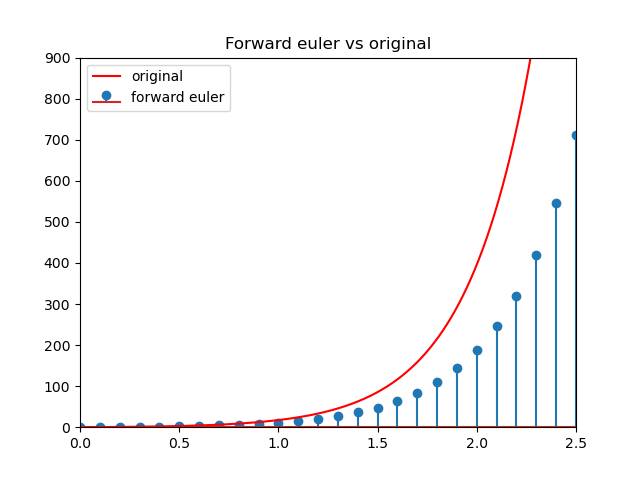
\includegraphics[width=0.7\textwidth]{figs/Euler.png}
    \caption{The plot depicting the divergence of forward euler from original at large values}
    \label{Plot of the function approaching the limit}
\end{figure} \newpage 
\end{enumerate}
\large\underline{{Python Implementation }}:
\begin{lstlisting}
codes/diff_eq.py
\end{lstlisting}
\end{enumerate}
%\end{document}
